\documentclass{article} % For LaTeX2e
\usepackage{iclr2018_conference,times}
\usepackage{url}
\usepackage{amsthm}
\usepackage{algorithm}
\usepackage{algorithmic}
\usepackage{times}
\usepackage{graphicx}
\usepackage{color}
\usepackage{amsmath}
\usepackage{amsfonts}
\usepackage{url}
\usepackage{textcomp}
\usepackage{amsthm}
\usepackage{float}

\frenchspacing

\def\presentationmode{1}

\def\beginFrame#1{\if\presentationmode1 \begin{frame}{#1} \else \fi}
\def\endFrame{\if\presentationmode1 \end{frame} \else \fi}

\newcommand{\mat}[1]{\mathrm{\mathbf{#1}}}
\newcommand{\vect}[1]{\mathrm{\mathbf{#1}}}
\newcommand{\fros}[1]{\left\| #1 \right\|_\mathrm{F}^2}
\newcommand{\Expect}[2]{\mathbb{E}_{#1}\left[ #2 \right]}
\newcommand{\KL}[2]{ \mathrm{KL}\left( #1 \| #2 \right) }
\newcommand{\Real}{\mathbb{R}}
\newcommand{\T}{\mathrm{T}}
\newcommand{\tr}{\mathrm{tr}}
\newcommand{\sigmoid}{\sigma}
\newcommand{\Simga}{\Sigma}
\newcommand{\attention}{\vect{g}}
\def\attentionwithouti{g_2, \dots, g_k}
%\def\attentionwithouti{\boldsymbol{\gamma}_{i}}
\newcommand{\attraction}{\vect{h}}

\def\x{\vect{x}}
\def\y{\vect{y}}
\def\h{\vect{h}}
\def\g{\vect{g}}
\def\s{\vect{s}}
\def\c{\vect{c}}
\def\A{\mathcal{A}}
\def\S{\mathcal{S}}
\def\R{\mathcal{R}}
\def\Trans{\mathcal{T}}
\def\E{\mathcal{E}}
\def\deriv#1#2{ \frac{\partial #2}{ \partial #1 } }
\def\derivN#1#2#3{ \frac{\partial^{#1} #3}{ \partial #2^{#1} } }
\def\grad#1#2{ \deriv{#1}{#2} }
\def\gradN#1#2#3{ \derivN{#1}{#2}{#3} }
\def\Grad#1#2{ \nabla_{#1} {#2} }
\def\obs{\vect{o}}
\def\u{{\boldsymbol{b}}}
\def\w{{\boldsymbol{\alpha}}}
\def\vmu{{\boldsymbol{\mu}}}
\def\v{\vect{v}}
\def\g{\attention}
\def\h{\attraction}
\def\G{\mat{G}}
\def\op{}
%\def\Qg{Q^{\mathrm{g}}}
%\def\ug{\vect{u}^{\mathrm{g}}}
\def\Qg{Q}
\def\ug{\u}
\def\params{{\boldsymbol{\theta}}}
\def\Params{{\boldsymbol{\Theta}}}
\def\opt#1{{\hat{#1}}}
\def\argmax{\mathrm{argmax}}

%\def\costof#1{C(#1)}
\def\costof#1{\mathrm{C}[{#1}]}
\def\budget{B}
\def\cost{c}
\def\vcost{\vect{\cost}}
\def\costat#1{\cost_{#1}}
\def\costi{c_i}
\def\unit{\vect{e}}
\def\units{k}
\def\state{\s}
\def\action{a}
\def\rewards{y}

\def\sumk#1{\sum_{#1=1}^k}
\def\Si{\sumk{i}}
\def\Sj{\sumk{j}}

\def\vcatout{\tilde{\vect{h}}}
\def\catout{\tilde{h}_i}
\def\catoutj{\tilde{h}_j}
\def\changeof#1{\Delta #1}

\def\vcatin{\vect{h}}
\def\catin{h_{i}}
\def\catinj{h_{j}}

\def\vcatbias{\vect{h}_i}
\def\catbias{\mu_i}
\def\catbiasj{\mu_j}

\def\qbias{q_i}
\def\vqbias{\mathbf{q}}
\def\qin{Q}

\def\ebias{e_{-i}}
\def\ein{e}
\def\changeofebias{{\changeof\qbias} \left[ \changeof\qbias + 2 \TDerror{\qin} \right]}
%\def\changeofebias{{\changeof\qbias}\left( \changeof\qbias + 2 \delta_t \right)}

\def\regret{\rho_{-i}}
%\def\TDerror#1{E_{\mathrm{TD}}\left({#1}\right)}
\def\TDerror#1{\delta}


\def\prA{p(\rewards|\state, \action, \params, \g)}
\def\LLAttention{\log \prA}

\def\Square#1{\left[ #1 \right]^2}

\def\ReplayMemory{\mathcal{D}}
\def\play{\s_t, a_t, r_t, \s_{t+1}}
\def\Play{(\play)}
\def\pl{\mathsf{d}_t}
\def\Replays#1{\Expect{ \pl \sim \ReplayMemory}{#1}}

\def\bUpdate#1{p(o_{t+1}|s_${#1},a_t) \sum_i p(s_{#1}|s_i, a_t) b_{t}^i}
\def\beliefState#1{ \vect{b}_{#1} }

\def\const{\mathrm{const.}}
\def\test{_\mathrm{test}}
\def\train{_\mathrm{train}}
\def\bs{\boldsymbol}
\def\etal#1{{et al.} (\citeyear{#1})}
\def\Etal{{et al.}}
\def\Long{1}
\def\eg{e.g., }

\def\eAt#1{e_{#1}}
\def\eBase{\eAt{\one}}
\def\one{\mathbf{1}}
\def\zero{\mathbf{0}}
\def\unit#1{\vect{u}_{#1}}
\def\eChange#1{ \Delta e_{#1} }

\def\ask{q}


% probability
\def\prob#1{p\left(#1\right)}
\def\prob#1#2{p\left(#1 \mid #2 \right)}

\def\deprecated{\alert{[Deprecated]}}
\def\softmax{\mathrm{softmax}}


\newcommand{\penalvec}[3]{ \frac{1}{2 \sigma_#1^2} \sum_{#2=1}^{#3} \vect{#1}_{#2}^\T  \vect{#1}_{#2} }

\newcommand{\CON}{\color{red}}
%\newcommand{\CON}{\color{black}}
\newcommand{\COFF}{\color{black}}

%\newcommand{\CON}{\color{red} -------- My modification starts from here. ------- \color{black}}
%\newcommand{\CON}{\color{black}}
%\newcommand{\COFF}{\color{red} -------- My modification ends here. ------- \color{black} }


\newtheorem{thm}{Theorem}[section]
\newtheorem{coro}{Corollary}[section]
\newtheorem{prf}{Proof}
\newtheorem{defn}{Definition}



\title{Neuron as an Agent}

%\author{Shohei Ohsawa, Kei Akuzawa, Yusuke Iwasawa \& Yutaka Matsuo \\
%The University of Tokyo\\
%7 Chome-3-1 Hongo, Bunkyo, Tokyo \\
%\texttt{ohsawa@weblab.t.u-tokyo.ac.jp} \\
%}
\author{Anonymous}

\newcommand{\fix}{\marginpar{FIX}}
\newcommand{\new}{\marginpar{NEW}}

\begin{document}

\maketitle

\begin{abstract}
Existing multi-agent reinforcement learning (MARL) communication methods have relied on a trusted third party (TTP) to distribute reward to agents, leaving them inapplicable in peer-to-peer environments. This paper proposes reward distribution using {\em Neuron as an Agent} (NaaA) in MARL without a TTP with two key ideas: (i) inter-agent reward distribution and (ii) auction theory. Auction theory is introduced because inter-agent reward distribution is insufficient for optimization. Agents in NaaA maximize their profits (the difference between reward and cost) and, as a theoretical result, the auction mechanism is shown to have agents autonomously evaluate counterfactual returns as the values of other agents. NaaA enables representation trades in peer-to-peer environments, ultimately regarding unit in neural networks as agents. Finally, numerical experiments (a single-agent environment from OpenAI Gym and a multi-agent environment from ViZDoom) confirm that NaaA framework optimization leads to better performance in reinforcement learning.
\end{abstract}

\section{Introduction}

%===========================================================================================
% Motivation
%===========================================================================================
After intelligence with reinforcement learning beat humans \citep{tesauro1995temporal,mnih2015human,silver2016mastering}, reinforcement learning has been expected to be applied into industry such as stock trade, autonomous cars, smart grid and IoT. 
In a world which realized the industrial application in the future, various types of companies will own their agents to improve their revenue.
The situation can be regarded as one that each agent are independently solving problems of partially observed Markov decision process (POMDP).

These agents in the companies are designed to maximize their own reward independently of each other. 
However, if the agents could exchange their own information, the entire revenue of the stakeholders would further increase.
As each agent has limited visibility of the environment, exchanging information among the agent will be helpful to solve their own tasks.
Thus, this paper aims to realize a society in which stakeholders which can have a conflict of interest trade their own information.
%Imagine diamond production with social division by different companies from raw material collection, processing to selling.
%If we can realize representation learning in the each layers as the social division, a single company can yield revenue more than one by itself. 

%in the case the company does it by itself.
%If the agents exchange their own information each other, entire revenue will be improved more than individuals.
%These agents in the companies are closed to maximize their own reward.
%Using economic metaphor, similarly to a supply chain of diamond from a company which collects raw material, one which processes it to one which sells it.
%Although agents in the companies are closed to maximize their own reward, if the agents exchange their own information each other, entire revenue will be improved more than individuals.

We regard the situation as communication in multi-agent reinforcement learning (MARL), addressed by several existing methods such as R/DIAL \citep{foerster2016learning} and CommNet \citep{sukhbaatar2016learning}.
CommNet is a state-of-the-art of MARL which considers communication among agents, 
and the feature is learning among agents with backpropagation.

In the case when we are trying to consider MARL in which different stakeholders make different agents which communicate each other, it needs design of incentive distribution (e.g., monetary payment) and a framework without {\em trusted third party} (TTP).
TTP \citep{wu1999game,sandholm2002possibility} is a neutral administrator which assumes distribution of reward for all the participants, supposed implicitly by most of existing literatures with regard to MARL \citep{agogino2006quicr,sukhbaatar2016learning,foerster2016learning,foerster2017counterfactual}.
While TTP is required to be neutral against all the participants,
several configuration of peer-to-peer trade such as inter-industry and -country trade cannot prepare TTP.
If untrusted third party assumes reward distribution, it can undesirably make reward for partial participants higher than necessity.

To the best of our knowledge, no existing literatures discuss the reward distribution on the configuration above.
Since CommNet assumes an environment which distributes a uniform reward to all the agents, 
in the case distributing limited reward in supply such as money, it causes {\em Tragedy of the Commons} \citep{lloyd1833two} in which contributing agents' reward will reduce due to participant of free riders.
Although there are several MARL methods which distributes reward depends on their contribution such as QUICR \citep{agogino2006quicr} and COMA \citep{sukhbaatar2016learning}, they suppose the existence of TTP, and hence it cannot be applied into our situation.

%===========================================================================================
% Objective
%===========================================================================================

Our proposed method, {\em Neuron as an Agent} (NaaA) extends CommNet to realize incentive distribution
in MARL without TTP with two key ideas: (i) inter-agent reward distribution and (ii) auction theory.
The reason why we introduce auction theory is inter-agent reward distribution is insufficient for optimization.
An agent in NaaA maximizes {\em profit}, difference between reward which it receives and cost which it redistributes to other agents.
If we optimize the framework naively, we obtain a trivial solution that agents make their cost zero to maximize the profit.
Then, NaaA employs game design with auction theory to keep cost being smaller than necessity.
As a theoretical result, we show that an agent autonomously evaluates {\em counterfactual return} as other agent's value.
Counterfactual return equals to discounted cumulative sum of counterfactual reward \citep{agogino2006quicr} which QUICR and COMA distribute.
NaaA realizes reward distribution which make it pareto improvement more than inter-agent reward distribution.

\begin{figure*}[tb]
	\centering
	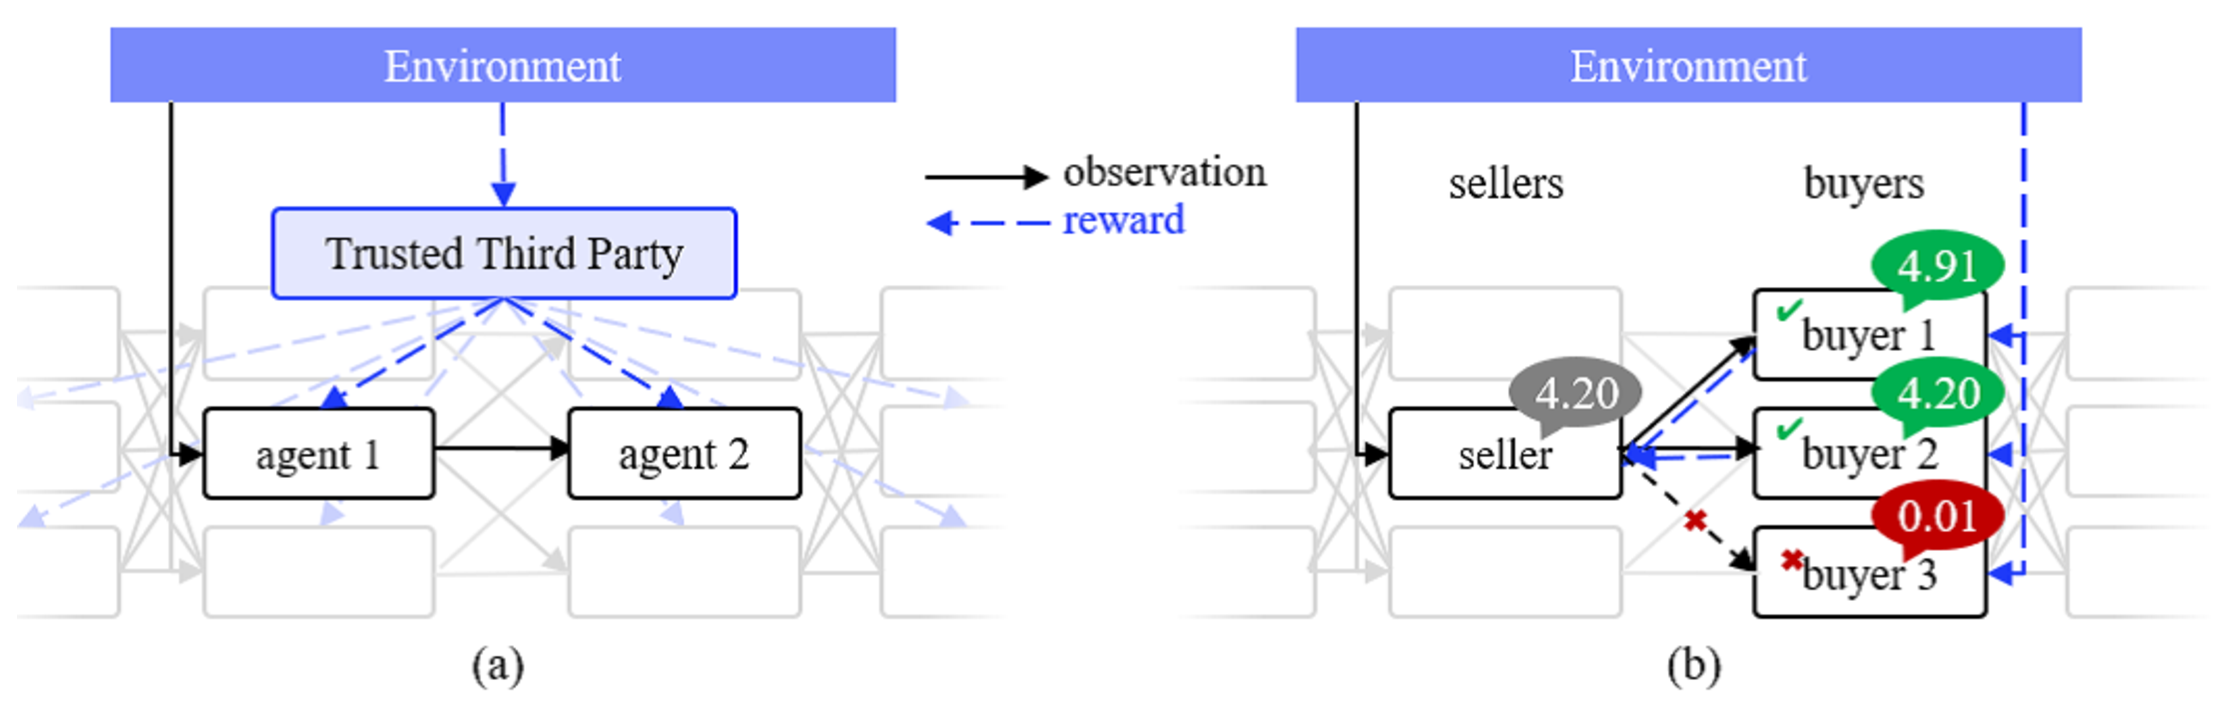
\includegraphics[width=\linewidth]{img/TTP.eps}
	\caption{
		A schematic illustration of reward disteribution models in MARL.
		{\bf (a)} Centralized reward distribution model \citep{agogino2006quicr,sukhbaatar2016learning,foerster2016learning,foerster2017counterfactual}
		{\bf (b)} Inter-agent reward distribution model (our model). Some agents receive reward from the environment directly,  
			and redistribute to other agents. The agents maximize their profit instead of reward.
		{\bf (c)} Neuron as an Agent (NaaA). Inter-agent reward distribution includes reward backpropagation along the connections. 
	}
	\label{fig:ttp}
\end{figure*}

NaaA enables us to trade of representation in peer-to-peer and regard a unit in a neural network as an agent ultimately.
As NaaA can regard a unit as an agent without loss of generality indeed, this paper uses the setting.
We illustrate the concept proposed method in \figurename~\ref{fig:ttp}.

In the experiment, we use an environment which extends ViZDoom \citep{kempka2016vizdoom}, a POMDP environemnt, to MARL.
We put two agents in the environment.
The one is a cameraman who send information, and the another one is a main player to defeat enemies with a gun.
We confirm that the cameraman learns cooperative action to send information in dead angle, behind of main player, and outperform CommNet in score.

Interestingly, NaaA can apply to a single-agent as well as multi-agent setting since it learns optimal topology between the units. %with respect to supervised learning
As a further application, we propose {\em Adaptive DropConnect} (ADC), which combines DropConnect \citep{wan2013regularization}, which randomly masks the topology, with an adaptive algorithm, which prunes connections with less counterfactual return with higher probability.
Experimental result in classification and reinforcement learning task shows ADC outperforms DropConnect.
%Subsequently, we present that our trading model leads the model to learning optimal topology between the units with respect to supervised learning as well as MARL.
%It uses $\varepsilon$-greedy as an exploration policy, and is equivalent to DropConnect in the case of $\varepsilon = 1$. It is equivalent to counterfactual return maximization, which constructs the topology deterministically in the case of $\varepsilon = 0$.

% Organization
The remaining part of this paper is organized as follows. 
First, we describe the two key ideas: inter-agent reward distribution and auction theory. 
After introducing related works, we show the experimental result in ViZDoom.
Next, we show ADC and its experimental result as a further application. 
Then, we conclude this paper.

\section{Problem Definition}
Suppose there is an $N$-agent system in an environment. 
The goal of this paper was to maximize the discounted cumulative reward the system obtained from the environment.
This was calculated as:
\begin{equation}
	G = \sum_{t=0}^T \gamma^t R_t^\mathrm{ex},
\end{equation}
where $R_{t}^\mathrm{ex}$ is a reward which the system obtains from the environment at $t$, 
and $\gamma \in [0, 1]$ is the discount rate and $T$ is the terminal time.

Reward distribution is distributing $R_t$ to all the agents under the following constraint.
\begin{equation}
	\sum_{i=1}^N R_{it} = R_t^\mathrm{ex},
	\label{eq:reward_const}
\end{equation}
where $R_{it}$ is a reward which is distributed to $i$-th agent at time $t$.
For instance, in robot soccer, the environment give a reward 1 when an agent shoot a ball to the goal.
Each agent should receive the reward along to their contribution.

%Trusted third party is required to calculate $R_{it}$.
In most of MARL communication methods, the policy of reward distribution is determined by a centralized agent.
For example, QUICR \citep{agogino2006quicr} and COMA \citep{foerster2017counterfactual} distribute $R_{it}$ according to counterfactal reward, difference of reward between an agent made an action and not.
The value of counterfactual reward is calculated by centralized agent, called {\em trusted third party} (TTP).

In a peer-to-peer environment such as inter-industry and -country trade, they cannot place a TTP. 
Hence, another framework required to actualize reward distribution without TTP.

\section{Neuron as an Agent}
%TODO: Show the figure.
% ���̏͂ł�������
% �E�j���[�������G�[�W�F���g�Ƃ݂Ȃ�
% �E�����‚��̑O����Ă���
% �ENaaA �� social welfare function ���ő剻���邱�Ƃ��A�O������̃����[�h�ő剻�Ɉ�v����B

\subsection{Problem Definition}
Suppose there are $N$ agents interacting to an environment. 
%This paper addresses reward distribution problem at multi-agent communication among the agents.
Some agents get reward from the environment, and distribute it to other agents as incentive to give precise information.
The reward is limited so that if an agent distribute $\rho$ reward, the agents' reward subtracted by $\rho$ such as currency.
For the reason, other agents for an agent itself can be interpreted as another environment which 
give a reward $-\rho$ instead of an observation $x$.
We name the another environment as {\em internal environment} and name the original environment as an {\em external environment}.

Our goal is to maximize the discounted cumulative reward which the system will obtain from the external environment.
 %total discounted cumulative reward from the external environment which all the $N$ agents will obtain.
\begin{equation}
%G^\mathrm{ex} = \sum_{i=1}^n \left[ \sum_{k=0}^T \gamma^k R_{i,k+t}^\mathrm{ex} \right],
G = \sum_{i=1}^n \left[ \sum_{t=0}^T \gamma^k R_{it}^\mathrm{ex} \right],
\end{equation}
where $R_{it}^\mathrm{ex}$ is an external reward which $i$-th agent obtains at $t$, and $\gamma \in [0, 1]$ is the discount rate and $T$ is the terminal time.

Similarly to CommNet \citep{sukhbaatar2016learning}, we assume that the communication protocol between the agent is a continuous quantity such as a vector, and the content can be trained by backpropagation.
Hence, we can interpret the multi-agent communication as a huge neural network.
Therefore, we can interpret a unit as an agent without loss of generality.
This framework can single-agent reinforcement learning as well as multi-agent reinforcement learning.

\subsection{The Framework}
A typical artificial neural network is a directed graph $\neuralnet = (\units, \edges)$ among the units.
$\units = \{\unitAt{1}, \dots, \unitAt{N}\}$ is a set of the units. $\edges \subset \units^2$ is a set of edges representing connections between two units.
If $(\unit, \unitAt{j}) \in \edges$, then connection $\unit \rightarrow \unitAt{j}$ holds, indicating that $\unitAt{j}$ observes activation of $\unit$.
We denote activation of the unit $\unit$ at time $t$ as $x_{it} \in \Real$.
Additionally, we designate a set of units which unit $i$ connects to as $\followers = \{j | (\unit, \unitAt{j}) \in \edges \}$ and a set of units which unit $i$ is connected from as $\followees = \{j | (\unitAt{j}, \unit) \in \edges \}$.
We denote $\friends = \followees \cup \followers$.

NaaA interprets $\unit$ as an agent.
Therefore, $\neuralnet$ is a multi-agent system.
An environment for $\unit$ comprises an environment that the multi-agent system itself touches and a 
set of the unit to which $\unit$ directly connects: $\{v_i \in \units | i \in \friends\}$.
We distinguish both environments by naming the former as an external environment, and by naming the latter as an internal environment.
$\unit$ will receive rewards from both environments.
We add the following assumption for characteristics of the $\unit$.
\begin{enumerate}
\renewcommand{\labelenumi}{N\arabic{enumi}:}
\item (Selfishness) 
	The utility which an $\unit$ wants to maximize is its own return (cumulative discounted reward):
	$G_{it} = \sum_{k=0}^T \gamma^k \rewardAt{i,t+k}$.
\item (Conservation) 	% Energy Conservation
	The summation of internal reward over $\units$ equals to 0.
	Hence, the summation of a reward by which $\units$ will receive both an internal and external environment $\reward$ are equivalent to reward $R_t^{\mathrm{ex}}$, which the entire multi-agent system receives from the external environment.
\item (Trade) 
	The $\unit$ receives internal reward $\rho_{jit}$ from $\unitAt{j} \in \units$ in exchange of activation signal $x_i$
	before transferring the signal to the unit. At the same time, $\rho_{jit}$ is subtracted from the reward of $v_j$.
\item (NOOP) 
	$\unit$ has NOOP (no operation), for which the return is $\delta > 0$ as an action.
	With NOOP, the unit inputs nothing and outputs nothing.
\end{enumerate}
In terms of neuroscience,
N1 states that the unit acts as a cell.
N2 and N3 state the distribution of NTF. N4 corresponds to apoptosis.
NOOP is selected when the expected returns of the other actions are non-positive.
In the following, we construct the framework of NaaA from the assumptions.

The social welfare function (total utility of the agents) $G^\mathrm{all}$ is equivalent to the objective function $G$. That is,
\begin{equation}
	G^\mathrm{all} = \sum_{i=1}^n G_{it} = \sum_{i=1}^n \left[ \sum_{k=0}^T \gamma^k R_{it} \right] 
		= \sum_{k=0}^T \left[ \gamma^k \sum_{i=1}^n R_{it} \right].
\end{equation}
From N2, $\sum_{i=1}^n R_{it} = \sum_{i=1}^n R_{it}^{\mathrm{ex}}$ holds. Hence, $G^\mathrm{all} = G$ holds.
%\begin{equation}
%	G^\mathrm{all} = \sum_{k=0}^T \left[ \gamma^k \sum_{i=1}^n R_{it}^{\mathrm{ex}} \right] = G.
%\end{equation}

%================================================================
\subsection{Cumulative Discounted Profit Maximization Framework}
%================================================================
We denote the external reward by which unit $\unit$ receives at time step $t$ as $R_{it}^\mathrm{ex}$, where $\sum_{i=1}^n R_{it}^\mathrm{ex} = R_t^{\mathrm{ex}}$ holds.
From N3, reward $R_{it}$, which $\unit$ receives at $t$ can be written as the following.
\begin{flalign}
	R_{it} = 
	  R_{it}^\mathrm{ex} + \sum_{j \in N^\mathrm{out}_i} \rho_{jit} 
	- \sum_{j \in N^\mathrm{in}_i} \rho_{ijt}.
\end{flalign}
The equation is divided into positive terms and a negative term, we name the former as revenue, and the latter as cost, and denote them respectively as $r_{it} = R_{it}^\mathrm{ex} + \sum_{j \in N^\mathrm{out}_i} \rho_{jit}, \, c_{it} = \sum_{j \in N^\mathrm{in}_i} \rho_{ijt}$.
We name $R_{it}$ as profit.


$\unit$ maximizes the cumulative discounted profit $G_{it}$ represented as
\begin{flalign}
	G_{it}	= \sum_{k=0}^T \gamma^k R_{i, t+k} 
			= \sum_{k=0}^T \gamma^k (r_{i,t+k} - c_{i,t+k})
			&= r_t - c_t + \gamma G_{i,t+1}.
\end{flalign}
$G_{it}$ is unobserved unless the time is reached at the end of the episodes.
Because prediction based on the current value is needed to select the optimal actions, 
we approximate $G_{it}$ with value function $V_i^{\pi_i} (s_{it}) = \Expect{\pi_i}{ G_{it} \mid s_{it}}$ where $s_{it} \in \Observations$.
In this case, the following equation holds.
\begin{flalign} 
		V_i^{\pi_i} (s_{it}) = r_{it} - c_{it} + \gamma V_i^{\pi_i} (s_{i, t+1}),	\label{eq:V}
\end{flalign}
Therefore, we need only consider maximization of revenue, the value function, and cost minimization.
$R_{it} > 0$, i.e., $r_{it} > c_{it}$ indicates that the unit gives the additional value to the obtained data.
The unit acts NOOP because $V_i^{\pi_i} (s_{it}) \leq 0 < \delta$ if $R_{it} \leq 0$ for all $t$ because of N4.

%TODO: verify equation of V



%The design of NaaA is inspired by neuroscience.
%A neuron in a neurocircuit consumes adenosine triphosphate (ATP) supplied from connected astrocytes.
%The astrocyte is a glia cell, which forms the structure of a brain. It supplies fuel from the vessel.
%Because the amount of ATP is constrained, the discarded neuron will become extinct with execution of apoptosis.
%Also, because apoptosis of a neuron is restrained by neurotrophins (NTFs) such as nerve growth factor (NGF) and brain-derived neurotrophic factor (BDNF),
%neurons which can obtain much NTF will live.
%The perspective of interpreting a neuron as an independent living object is known as neural Darwinism \citep{edelman1987neural}.

\section{Related Work}
NaaA belongs to a class of partially observable stochastic game (POSG) \citep{hansen2004dynamic} because it processes multiple units as agents.
POSG, a class of reinforcement learning with multiple agents in a POMDP environment, presents several research issues, one of which is communication.
CommNet \citep{sukhbaatar2016learning}, which exploits the characteristics of a unit that is agnostic to the topology of other units, employs backpropagation to train multi-agent communication.
Another one is credit assignment.
Instead of reward $R(a_t)$ of an agent $i$ for actions at $t$ $a_t$, 
QUICR-learning \citep{agogino2006quicr} maximizes counterfactual reward $R(a_t) - R(a_t - a_{it})$, the difference in the case of the agent $i$ takes an action $a_{it}$ ($a_t$) and not ($a_t-a_{it}$).
COMA \citep{foerster2017counterfactual} also maximizes counterfactual rewards in an actor--critic setting.
In the setting, all actors have common critics, which improves both actors and critics with time difference (TD)-error of a counterfactual reward.
This paper unifies both issues: communication and credit assignment.
The main proposal is a framework to manage the agents to maximize the {\em counterfactual return}, the extended counterfactual reward along the time axis.

Training a neural network with a multi-agent game is an emerging methodology.
Generative adversarial nets (GAN) \citep{goodfellow2014generative} have the goal of obtaining true generative distribution as a Nash equilibrium of a competitive game that includes two agents with contradictory rewards: a generator and a discriminator. 
In game theory, the outcome maximizing overall reward is named Pareto optimality.
Nash equilibrium is not guaranteed to converge to Pareto optimality. The difference between them is designated as a dilemma.
Because the existence of a dilemma depends on the reward design, methods to resolve dilemmas with good reward design are being investigated: mechanism design \citep{myerson1983mechanism} is also known as inverse game theory.
Mechanism design is applied to auctions \citep{vickrey1961counterspeculation} and matching \citep{gale1962college}.
GAN and our proposal, NaaA, are outcomes from mechanism design.
NaaA applies a digital goods auction \citep{guruswami2005profit} to reinforcement learning with a multi-agent neural network, 
to obtain a maximized return by units as a Nash equilibrium.

Adaptive DropConnect (ADC) which we propose in a late part of this paper, extends DropConnect \citep{wan2013regularization}, a regularization technique.
The idea of ADC (instead of dropping each connection between the units in constant probability, using skew probability correlated to absolute value of weights) is eventually closer to Adaptive DropOut \citep{ba2013adaptive} although the derivation is different, 
and the adjective ``adaptive'' is added respecting the method.
Optimizing neural network with RL is investigated by \cite{andrychowicz2016learning}.
In contrast to their methods which uses recurrent neural network (RNN) and hence the implementation is difficult,
our method is RNN-free and forms as a layer, and hence the implementation is easy and fast, and it has wide applicable area.

\section{Experiment}
To confirm that NaaA works widely with machine learning tasks, we confirm our method of supervised
learning tasks as well as reinforcement learning tasks. As supervised learning tasks, we use
typical machine learning tasks such as image classification using MNIST, CIFAR-10, and SVHN.

As reinforcement tasks, we confirm single- and multi-agent environment. The single-agent environment
is from OpenAI Gym. We confirm the result using a simple reinforcement task: CartPole. In
multi-agent, we use ViZDoom, a 3D environment for reinforcement learning.

\subsection{Classification}
\subsubsection{Setup}
%This experiment verified the performance of two tasks: classification and single-agent reinforcement learning.
For classification, three types of datasets were used: MNIST, CIFAR-10, and STL-10. 
The given task was to predict the label of each image, and each dataset had a class number of 10.
The first dataset, MNIST, was a collection of black and white images of handwritten digits sized 28�~28. The training and test sets contained 60,000 and 10,000 example images, respectively. 
The CIFAR-10 dataset images were colored and sized 32�~32, and the assigned task was to predict what was shown in each picture. This dataset contained 6,000 images per class (5,000 for training and 1,000 for testing).
The STL-10 dataset was used for image recognition, and had 1,300 images for each class (500 training, 800 testing). Each image was sized 96�~96; however, for the experiment, the images were resized to 48�~48 because the greater resolution of this dataset (relative to the above datasets) required far more computing time and resources.

\subsubsection{Model}
Two models were compared in this experiment: DropConnect and Adaptive DropConnect (the model proposed in this paper). The baseline model was composed of two convolutional layers and two fully connected layers whose outputs are dropped out (we set the possibility as 0.5). The labels of input data were predicted using log-softmaxed values from the last fully connected layer. In the DropConnect and Adaptive DropConnect models, the first fully connected layer was replaced by a DropConnected and Adaptive DropConnected layer, respectively. It should be noted that the DropConnect model corresponded to the proposed method when $\varepsilon$ = 1.0, meaning agents did not perform their auctions but instead randomly masked their weights.

\subsubsection{Results}
The models were trained over ten epochs using the MNIST datasets, and were then evaluated using the test data. The CIFAR-10 and STL-10 epoch numbers were 20 and 40, respectively. Experiments were repeated 20 times for each condition, and the averages and standard deviations of error rates were  calculated. Results are shown in Table \ref{tbl:cls}. As expected, the Adaptive DropConnect model performed with a lower classification error rate than either the baseline or DropConnect models regardless of the given experimental datasets.


\begin{table}[h]
	\caption{ Experimental result for image classification tasks and single-agent RL }\label{tbl:cls}. 
\centering
\begin{tabular}{l|ccc|c}
\hline
		& MNIST & CIFAR-10 & STL-10 & CartPole \\
\hline
		DropConnect \citep{wan2013regularization}	&	1.72 $\pm$ 0.160	&	43.14 $\pm$ 1.335	&	50.92 $\pm$ 1.322 & 285 $\pm$ 21.5 \\
		Adaptive DropConnect	&	\textbf{1.36} $\pm$ 0.132	&	\textbf{39.84} $\pm$ 1.035	&	\textbf{42.17} $\pm$ 2.329 & \textbf{347} $\pm$ 29.4 \\
\hline
\end{tabular}
\end{table}

\subsection{Single-agent RL}
Next, the single-agent reinforcement learning task was set as 
the CartPole task from OpenAI Gym \citep{openaigym} with visual inputs.
In this setting, the agent was required to balance a pole while moving a cart.
The images contained a large amount of non-useful information, making pixel pruning important.
The result in Table \ref{tbl:cls} demonstrates that our method improves the standard RL.

\subsection{Multi-agent RL}
The proposed reward distribution method was confirmed to work as expected by a validation experiment using the multi-agent setting in ViZDoom \citep{kempka2016vizdoom}, 
an emulator of Doom containing a map editor where additional agents complement the main player.
A main player in the ViZDoom environment aims to seek the enemy in the map and then defeat the enemy.

\subsection{Setup}
A defend the center (DtC)-based scenario, provided by ViZDoom platform, was used for this experiment.
Two players, a main player and a cameraman, were placed in the DtC, where they started in the center of a circular field and then attacked enemies that came from the surrounding wall.
Although the main player could attack the enemy with bullets, 
the cameraman had no way to attack, only scouting for the enemy.
The action space for the main player was the combination of \{ attack, turn left, turn right \}, giving a total number of actions $2^3 = 8$.
The cameraman had two possible actions: \{ turn left, turn right \}.
Although the players could change direction, they could not move on the field.
Enemies died after receiving one attack (bullet) from the main player, and then player received a score of +1 for each successful attack.
The main player received 26 bullets by default at the beginning of each episode.
The main player died if they received attacks from the enemy to the extent that their health dropped to 0, and received a score of -1 for each death.
The cameraman did not die if attacked by an enemy.
Episodes terminated either when the maim player died or after 525 steps elapsed.

\subsection{Model}
Three models, described below, were compared: the proposed method and two comparison targets.

{\em Baseline}: DQN without communication. The main player learned standard DQN with the perspective that the player is viewing.
Because the cameraman did not learn, this player continued to move randomly.

{\em Comm}: DQN with communication, inspired by Commnet. The main player learns DQN with two perspectives: theirs and that of the cameraman.
The communication vector is learned with a feed-forward neural network.

{\em NaaA}: The proposed method. The main player learned DQN with two perspectives: theirs and that of the cameraman.
Transmissions of rewards and communications were performed using the proposed method.

\begin{figure*}[t]
\centering
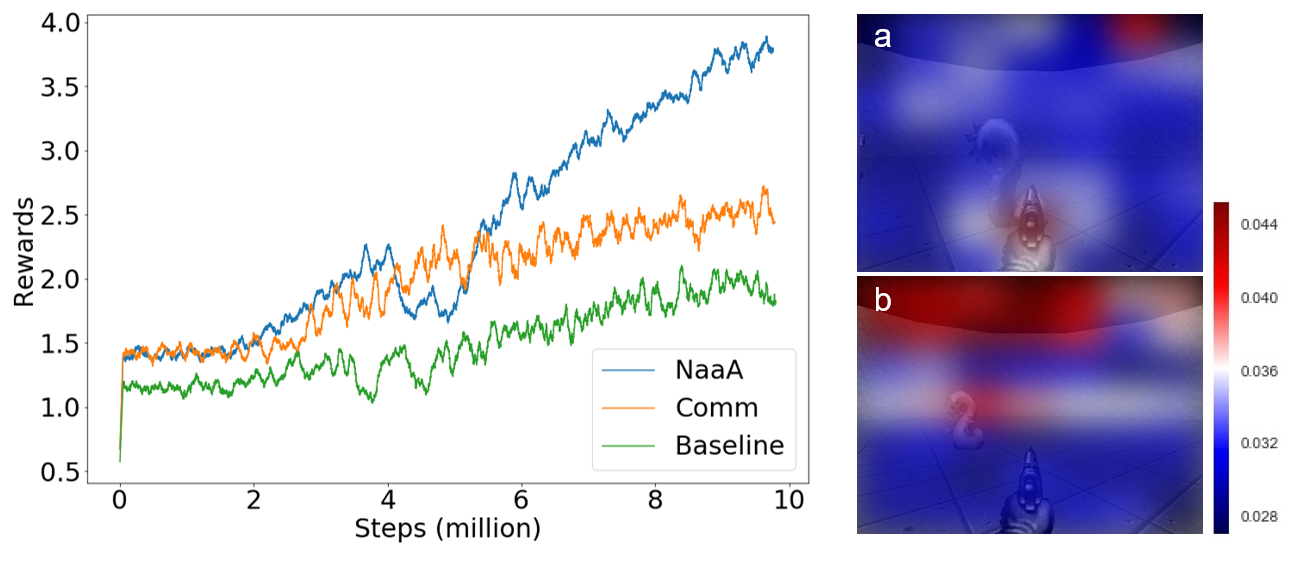
\includegraphics[width=\linewidth]{img/lc_vis.eps}
\caption{
	\textbf{Left:}
		Learning curve for ViZDoom multi-agent task. 
		The proposed NaaA--based method outperformed the other two methods (baseline and Comm DQNs).
	\textbf{Right:} 
		Visualizing reward from the main player to the cameramann shows us what is important information for the main player:
		(a) The pistol.
		(b) The point at which the enemy appeared and approached.
}
\label{fig:lc_vis}
\end{figure*}

\begin{figure*}[t]
\centering
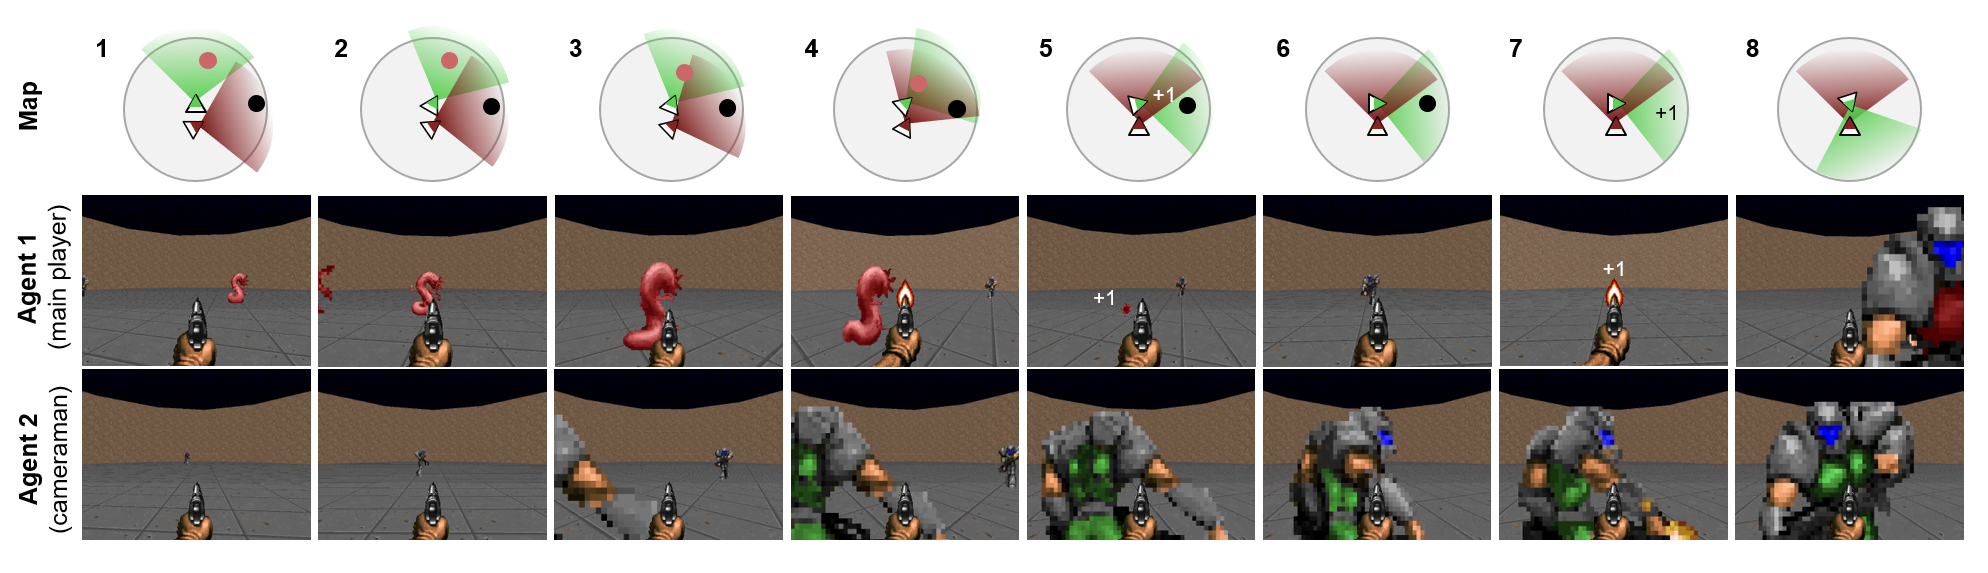
\includegraphics[width=\linewidth]{img/circleworld.eps}
\caption{
NaaA leads agents to enter a cooperative relationship.
First, the two agents face different directions,
and the cameraman sells their information to the main player (\textbf{1}).
The main player (information buyer) starts to turn right to find the enemy.
The cameraman (information seller) starts to turn left to seek new information by finding the blind area of the main player (\textbf{2} and \textbf{3}).
After turning, the main player attacks the first, having already identified enemy (\textbf{4} and \textbf{5}).
Once the main player finds the enemy, he attacks and obtains the reward (\textbf{6} and \textbf{7}).
Both agents then return to watching the dead area of the other until the next enemy appears (\textbf{8}).
}
\label{fig:circleworld}
\end{figure*}

\subsection{Results}
Training was performed over the course of 10 million steps.
Figure \ref{fig:lc_vis} Left demonstrates the proposed NaaA model outperformed the other two methods.
Improvement was achieved by Adaptive DropConnect.
It was confirmed that the cameraman observed the enemy through an episode, which could be interpreted as the cameraman reporting enemy positions.
In addition to seeing the enemy, the cameraman observed the area behind the main player several times.
This enabled the cameraman to observe enemy attacks while taking a better relative position.

To further interpret this result, 
a heatmap visualization of revenue earned by the agent is presented in Figure \ref{fig:lc_vis} Right.
The background picture is a screen from Doom, recorded at the moment when the CNN filter was most activated.
%The center corresponds to a position with the enemy appearing far away.
%The top corresponds to a position with the enemy coming closer.
%(b) shows that the agent sees the pistol.
Figure \ref{fig:circleworld} shows an example of learnt sequence of actions by our method.


%To confirm that NaaA works widely with machine learning tasks,
%we confirm our method of supervised learning tasks as well as reinforcement learning tasks.
%As supervised learning tasks, we use typical machine learning tasks such as image classification
%using MNIST, CIFAR-10, and SVHN.

%As reinforcement tasks, we confirm single- and multi-agent environment.
%The single-agent environment is from OpenAI gym.
%We confirm the result using a simple reinforcement task: CartPole.
%In multi-agent, we use ViZDoom, a 3D environment for reinforcement learning.

%The additional feature of NaaA is credit assignment for reward distribution, 
%meaning that if the neural network is divided into multiple agents, it works by playing the auction game.


%\section{Conclusion and Future Works}
\section{Concluding Remarks and Future Work}
This paper proposed a NaaA model to address communication in MARL without a TTP based on two key ideas: inter-agent reward distribution and auction theory.
Existing MARL communication methods have assumed the existence of a TTP, and hence could not be applied in peer--to--peer environments.
The inter-agent reward distribution, making agents redistribute the rewards they received from the internal/external environment, was reviewed first.
When an envy-free auction was introduced using auction theory, it was shown that agents would evaluate the counterfactual returns of other agents.
The experimental results demonstrated that NaaA outperformed a baseline method and a CommNet-based method.

Furthermore, a $Q$-learning based algorithm, termed Adaptive DropConnect, was proposed to dynamically optimize neural network topology with counterfactual return evaluation as a further application.
To evaluate this application, experiments were performed based on a single-agent platform, demonstrating that the proposed method produced improved experimental results relative to existing methods.

% TODO: ���������ꍇ�̑΍�͂ǂ����ɏ���������������������Ȃ�

Future research may also be directed toward considering the connection between NaaA and neuroscience or neuroevolution.
Edeleman propounded the concept of neural Darwinism \citep{edelman1987neural}, in which group selection occurs in the brain.
Inter-agent rewards, which were assumed in this paper, correspond to NTFs
and could be used as a fitness function in genetic algorithms for neuroevolution such as hyperparameter tuning.

As NaaA can be applied in peer-to-peer environments, 
the implementation of NaaA in blockchain \citep{swan2015blockchain} is under consideration.
This implementation would extend the areas where deep reinforcement learning could be applied.
Bitcoin \citep{nakamoto2008bitcoin} could be used for inter-agent reward distribution, and the auction mechanism could be implemented by smart contracts \citep{buterin2014next}.
Using the NaaA reward design, it is hoped that the world may be united, allowing people to share their own representations on a global scale.

%We can use bitcoin \cite{nakamoto2008bitcoin} and smart contract \cite{}a 

%Besides, we proposed Adaptive DropConnect as an further application on a single neural network.
%This paper proposed NaaA, a reinforcement learning framework that treats each unit on a neural network as an agent.
%First, we pointed out there are dilemma problems if we naively optimize NaaA. 
%We proposed an optimization method with auction.
%Consequently, an action by which units evaluate the counterfactual return of other units is obtained as a Nash equilibrium.
%Furthermore, we proposed $Q$-learning based algorithm, adaptive dropconnect, to optimize the neural network topology dynamically with evaluation of counterfactual return.
%For the evaluation, we performed experiments based on single-agent and multi-agent platforms, demonstrating that our experimentally obtained results improve existing methods.

%As a direction of future research, we use on-policy methods to perform adaptive dropconnect, and
%consider applications combining genetic algorithms.

\bibliography{daisy}
\bibliographystyle{iclr2018_conference}

\appendix
\section*{Appendix}

% Set numbering of section alphabet: A, B, C,...
\setcounter{section}{1}
\renewcommand{\thesection}{\Alph{section}}

% Contents is started from here
%\subsection{Proof}
%We first proof $\rho_{ijt} = 0$ is the Nash equilibrium.
%The value function can be written as $r_{it} - c_{it} + \gamma V_{i,t+1}$.
%At the point, as other agents plays $\rho_{ijt} = 0$, the value function is $- c_{it}$.
%To maximizing this equation, $\rho_{ijt} = 0$ holds. 

\subsection{Proof of Theorem \ref{thm:optimal-bidding}}
As for a buyer, the asking price $\ask$ for a seller is unknown,
we address $\ask$ which has support $[0, \infty)$,
and consideration to maximize $\Expect{q}{G(b,q)}$,
In this case, the following equation holds.
\begin{flalign}
\deriv{b}{}\Expect{q}{G(b,q)} 
&= \deriv{b}{}\int_0^\infty (H(b - q) \cdot (v-q) + G_0) p(q) dq \notag \\
&= \deriv{b}{} \left[ \int_0^b (v-q) p(q) dq + G_0 \int_0^\infty p(q)dq \right] \notag \\
&= \deriv{b}{} \int_0^b (v-q) p(q) dq \notag \\
&= (v-b) p(q=b), \notag 
\end{flalign}
Therefore, the condition to maximize $\Expect{q}{G(b,q)}$ is $b=v$.


\end{document}
